%% -----------------------------------------

%% Vorlesungsmitschrift (Kapitel 4)

%% an der Uni Regensburg, gelesen von Christian Back

%% -----------------------------------------


\chapter{Elektromagnetische Wellen an Grenzflächen}
\section{Randbedingungen der elektromagnetischen Welle}
Wir wollen jetzt Wellenausbreitung in inhomogenen Medien beschreiben, z.B. den Übergang von Medium 1 nach Medium 2, also einer Grenzfläche.
\paragraph{Randbedingungen der MWGl.:} Die Tangentialkomponenten von $\vecE$ und $\vecH=\fracone{\muo\mu_r}\vecB$ sind stetig. Die Normalkomponenten von $\vecD=\epso\eps_r\vecE$ und $\vecB$ sind ebenfalls stetig. (isotrope, isolierende, nicht magnetische Medien $\mu=1$)
\paragraph{einfachster Fall:}zwei homogene Medien mit Brechungsindex $n_e$ (einfallender Strahl) und $n_t$ (transmittierte Welle).
% 
% Skizze zu Reflexion
% 
Der Winkel $\alpha$ liegt zwischen $\veck_e$ und $\vece_y$ bzw. zwischen $\veck_t$ und $\vece_y$. Wir nehmen an, dass es eine fest vrogegebene einlaufende Welle ist.
\begin{align*}
  \vecE_e&=\vecE_{e_0}cor(\omega_et-\veck_e\vecr)=\vecE_{e_0}(\phi_e(\vecr,t))\\
  \vecE_r&=\vecE_{r_0}cor(\omega_rt-\veck_r\vecr+\varphi_r)=\vecE_{r_0}(\phi_r(\vecr,t))\\
  \vecE_t&=\vecE_{t_0}cor(\omega_tt-\veck_t\vecr+\varphi_t)=\vecE_{t_0}(\phi_t(\vecr,t))
\end{align*}
Die Wellenvektoren $\veck_e,\veck_r$ und $\veck_t$ müssen die Dispersionsrelationen im jeweiligen Medium erfüllen. Die Phasenfaktoren $\varphi_r,\varphi_t$ bestimmen die Phasenlage relativ zur einlaufenden Welle.
% -----------------------------
% Vorlesung vom 2.11 fehlt hier
% -----------------------------

% -----------------
% 04.11.2015

\begin{description}
\item[$n_e>n_t$:] Wenn Licht von optisch dichteren in ein optisch dünneres
  Medium übergeht, ist der Reflexionskoeffizient größer null. 
  Daraus folgt, dass $\vecE_{0r}$ und $\vecE_{0e}$ in die gleiche
  Richtung zeigen und die Wellen an der Grenzschicht in Phase sind. 
\item[$n_e<n_t$:] Wenn Licht aus einem optisch dünneren in ein optisch dichteres
  Medium übergeht, wird der Reflexionskoeffizient kleiner Null und
  $\vecE_{0r}$ und $\vecE_{0e}$ zeigen in antiparallele Richtungen
  Außerdem liegt bei der Reflexion ein Phasensprung von $\pi$ vor,
  bei Transmission aber nicht.
\end{description}
Da die reflektierte Intensität nur proportional zu
$|\vecE|^2$ ist, spielt der Phasenfaktor keine Rolle.

\minisec{Reflexionsgrad%
\nomenclature{$R$}{Reflexionsgrad}%
\index{Reflexionsgrad}
der Intensität}
\begin{gather*}
  R = \frac{I_r}{I_e}
  =\left( \frac{n_e-n_t}{n_e+n_t} \right)^2
  =\left( \frac{n_{et}-1}{n_{et}+1} \right)^2
  =\left( \frac{1-n_{te}}{1+n_{te}} \right)^2
\end{gather*}
Der Reflexionsgrad ist unabhängig davon, von welcher Seite das Licht
einfällt. Er hängt allein von der Änderung des relativen
Brechungsindex ab. Wird das Licht aber absorbiert, wird der
Reflexionskoeffizient komplex und kann geschrieben werden als
\begin{align*}
  R=\vert r\vert^2=rr^*
\end{align*}
\paragraph{Beispiel:}
\begin{center}
  \begin{tabular}{lll}
    \emph{Übergang} & \emph{relativer Brechungsindex} & \emph{Reflexion in \%}\\
    Luft -- Glas & \num{1.5} & \SI{4}{\percent} \\
    Luft -- Diamant & \num{2.41} & \SI{17}{\percent}
  \end{tabular}
\end{center}

\subsection[Beliebige Einfallswinkel]{Beliebige Einfallswinkel $\alpha$}
Zunächst betrachten wir ein $\vecE$-Feld, das parallel zur
Einfallsebene schwingt und p"=polarisiert (d.\,h. parallel zur Einfallebene)
ist. Im Folgenden werden die Tangentialkomponenten mit dem Index~$T$
versehen und die Normalkomponenten mit dem Index~$N$. Betrachte außerdem
noch die Setigkeitsbedingungen für $\vecE$ und
$\vecD=\epso\eps\vecE$.
\begin{align*}
  E_{eN} &= E_e\sin\alpha
  &E_{tN} &= E_t\sin\beta
  &E_{rN} &= E_r\sin\alpha\\
  E_{eT} &= E_e\cos\alpha
  &E_{tT} &= E_t\cos\beta
  &E_{rT} &= -E_r\cos\alpha
\end{align*}
% ------------------------------------------------------------------------------
% Hab mir hier die Herleitung gespart oder sollen wir sie doch noch
% mit rein nehmen? 
% ------------------------------------------------------------------------------
Mit Hilfe der Stetigkeitsbedingungen und der Snellschen Formel,
erhalten wir daraus die 
\emph{Fresnelschen Formeln}\index{Fresnelsche Formeln}, 
Wobei $r_p$ der Reflexionskoeffizient für p"=polarisiertes Licht ist. 
\begin{align}
  r_{\parallel} 
  &= r_p
    = \frac
    {n_t\cos\alpha - n_e\cos\beta}
    {n_t\cos\alpha + n_e\cos\beta}
    = \frac
    {\tan(\alpha - \beta)}
    {\tan(\alpha + \beta)}\label{FF1}\\
  r_{\bot}
  &=r_s
    = \frac
    {n_e\cos\alpha - n_t\cos\beta}
    {n_e\cos\alpha + n_t\cos\beta}
    = -\frac
    {\sin(\alpha - \beta)}
    {\sin(\alpha + \beta)}\label{FF2}
\end{align}
Die Amplituden der reflektierten $\vecE$-Felder erhält man durch
Multiplikation der Amplituden des emittierten $\vecE$-Felder mit den
Reflexionskoeffizienten.


\minisec{Transmittierte Leistung $P_t$%
\nomenclature{P_t}{transmittierte Leistung}%
\index{transmittierte Leistung} 
und Intensität $I_t$%
\nomenclature{I_t}{transmittierte Intensität}%
\index{transmittierte Intensität}}
Wenn man nicht direkt an den Amplituden sondern an der
Leistung interessiert ist, kann man diese auch über den
Transmissionsgrad $T^P=\frac{P_t}{P_e}$ 
(bzw. bei der Intensität
$T^{I}=\frac{I_t}{I_e}$%
\index{Transmissionsgrad}%
\nomenclature{T^P}{Transmissionsgrad der Leistung; 
  $T^P=\frac{P_t}{P_e}$}%
\nomenclature{T^I}{Transmissionsgrad der Intensität;
  $T^{I}=\frac{I_t}{I_e}$})
berechnen. Aufgrund der Energieerhaltung gilt $P_e=P_r+P_t$ und man
erhält
\begin{gather*}
  T_{\parallel}^P = 1-\vert r_{\parallel}\vert^2
  \qquad\text{sowie}\qquad
  T_{\bot}^P = 1-\vert r_{\bot}\vert^2
\end{gather*}
Für die Berechnung der Intensität ist allerdings die Änderung der
Fläche zu berücksichtigen, da sich die Ausdehnung des Lichtstrahls auf
der Einfallebene und im transmittierten Strahl ändert.
\begin{align*}
  d^\prime &= \frac{d}{\cos\alpha}
  &d_t &= d^\prime\cos\beta 	
\end{align*}
Nun kann man folgende Gleichungen formulieren
\begin{align*}
  T^p &=\frac{P_t}{P_e}
        =\frac{I_t A_t}{I_e A_e}
        =\frac{I_t \cos\beta}{I_e\cos\alpha}
        =\frac{n_t |t|^2 \cos\beta}{n_e\cos\alpha}\\
  T^{I}&=\frac{I_t}{I_e}
         =T^P\frac{\cos\alpha}{\cos\beta}
         = |t|^2\frac{n_t}{n_e}
\end{align*}

\subsubsection{Diskussion der Fresnel'schen Formeln: Reflexionsgrad bei Lichteinfall aus einem optisch dünnerem Medium}
Ein Beispiel hierfür ist der Übergang von Luft in Gas mit $\frac{n_t}{n_e}=1,5$.
Betrachte nun die Winkelabhängigkeit von $R=\vert r\vert^2$ aus den
Fresnel'schen Formeln \ref{FF1} und \ref{FF2}. 
Bei Erhöhung des Winkels steigt $R_{\bot}$ stetig von \SI{4}{\percent}
bis \SI{100}{\percent} an. 
$R_{\parallel}$ sinkt hingegen anfangs bis zu einem gewissen Winkel
auf Null ab. Dieser Winkel wird auch
\emph{Brewsterwinkel}%
\nomenclature{$\alpha_B$}{Brewsterwinkel; 
  Winkel, bei dem reflektierter und gebrochener Strahl senkrecht
  aufeinander stehen; 
  Winkel vollständiger linearer Polarisierung bei Reflektion;
  $\tan\alpha_B = \frac{n_t}{n_e}$}%
\index{Brewsterwinkel} 
genannt, danach steigt
$R_{\parallel}$ ebenfalls auf die \SI{100}{\percent} an (siehe
Abb.\ref{RefGrad}).
\begin{figure}
  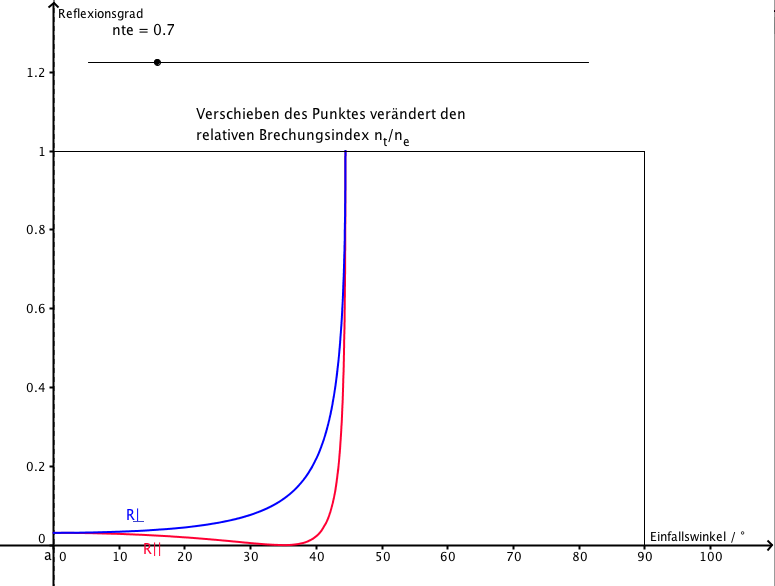
\includegraphics[width=\linewidth]{Bilder/Reflexionsgrad}
  \caption{Reflexionsgrad in Abhängigkeit des Einfallwinkels\label{RefGrad}}
\end{figure}
Der Brewsterwinkel $\alpha_B$ oder auch $\alpha_P$ wird dann erreicht,
wenn der Nenner divergiert, also $\tan(\alpha_B+\beta)=\infty$
bzw. $\alpha+\beta=90\degree$. In diesem Fall stehen der reflektierte
und der gebrochene Strahl aufeinander senkrecht.
Dies lässt sich wie folgt erklären. Man nehme an, dass der
reflektierte Strahl durch einen oszillierenden Dipol mit Dipolmoment
parallel zum $\vecE$-Feld in der Grenzschicht erzeugt wird. Dabei ist
die abgestrahlte Leistung $P(\theta)\propto\sin^2\theta$ und $\theta$
ist der Winkel zwischen Wellenvektor des abgestrahlten Lichts und
Dipolachse. Also wird längs zur Dipolachse ($\theta=0$) kein Licht
abgestrahlt -- $\vecE_{\parallel}$ wird nicht reflektiert. 
\emph{Daraus kann man folgern, dass das Licht vollständig linear
  polarisiert ist.}
Der Brewsterwinkel ergibt sich aus der Formel
\begin{align*}
  \tan\alpha_B &= \frac{n_t}{n_e}
\end{align*}

% 
% Vorlesung vom 9.11
% ------------------ 

\subsection{Absorbierende Medien}
Das Reflexionsvermögen bei absorbierenden Medien ist mit
Fresnelformeln ebenfalls berechenbar. 
Man ersetze nur $n$ durch seine komplexe Darstellung $n_R+in_I$. Nun
erhält man einen komplexen Reflexionskoeffizient und
Reflexionsgrad:
\begin{align*}
  r &= \frac{n_{rel}-1}{n_{rel}+1}\\
  R &= rr^*=\frac{(n_R-1)^2+n_I^2}{(n_R+1)^2+n_I^2}
\end{align*}
Daraus ergibt sich allgemein
\begin{itemize}
\item Das Reflexionsvermögen nimmt mit steigender Absorption
  zu (z.\,B. ideal leitende Metalle $\omega<\omega_p$). Bei Spiegeln
  ist beispielsweise $R\approx100\%$ im Infrarot (IR), Nahinfrarot
  (NIR) und im sichtbaren Bereich (VIS), wobei $R$ im sichtbaren
  Breich bereits zurück geht.
\item Mit wachsender Absorption ($n_I$ bzw. $k$) verschwindet der Brewsterwinkel, es bleibt ein Minimum von $R_{\parallel}$
\item Die Farbe von Gegenständen hängt von den dielektrischen Eigenschaften ab.
\end{itemize}

Verwendet man im sichtbaren Bereich ein weißes Licht mit allen
Spektralanteilen, lässt sich das Erscheinungsbild verschiedener
Materialien durch Reflexion, Transmission und Absorption beschreiben:
\begin{description}
\item[Metalle] sind durch ihre hohe Leitfähigkeit
  charakterisiert, die sich in einer spektral breitbandigen Reflexion
  äußern. Dadurch entsteht der metallische Glanz.
\item[Isolatoren, die im VIS-Bereich keine Absorption besitzen,]
  sind transparent. Allerdings wenn ihre Oberfläche gestört wird,
  werden sie weiß aufgrund ihres wellenlängenunabhänigem
  Reflexionsvermögen (vgl. Zucker -- Puderzucker). 
\item[Isolatoren mit nur einer schwachen Absorption] im VIS-Bereich
  zeigen in Transmission und Reflexion jeweils andere Farben. Dies
  wird durch die spektrale Verteilung des transmittierten Lichts
  bestimmt (vgl. verdünnte Tinte). 
\item[Isolatoren mit sehr hoher Absorption] -- also sehr hoher
  Reflexion -- haben eine Transmissionsfarbe, die wieder durch den
  Spektralbereich mit optimaler Transparenz bestimmt.
\end{description}



%%% Local Variables:
%%% mode: latex
%%% TeX-master: "../OptikSkriptWS1516"
%%% End:
